\documentclass[12pt,letterpaper,titlepage]{article}

\usepackage{fontspec}
\defaultfontfeatures{Mapping=tex-text}
\usepackage{xunicode}
\usepackage{xltxtra}
\usepackage{amsmath}
\usepackage{pdfpages}
\usepackage{amsfonts}
\usepackage{bbold}
\usepackage{amssymb}
\setcounter{secnumdepth}{0}
\usepackage{nameref}
\usepackage{enumitem}
\usepackage{environ}
\usepackage{pgfplots}

\showboxdepth=\maxdimen
\showboxbreadth=\maxdimen


\usepackage{paracol}
\usepackage{wrapfig}
\globalcounter{table}
\globalcounter{figure}
\usepackage{graphicx}
\usepackage[left=1in,right=1in,top=1in,bottom=1in]{geometry}
\graphicspath{{img/}}

\author{Jacob Abel}
\title{	Design \& Simulate 7 Ex2.1
	\\\large ECE2204 CRN:82929
}

\setlength{\parskip}{0.5em}

\begin{document}
\maketitle
\begin{raggedright}

\section{Problem 7.2-1.a.1: }
\subsection{Design}
Determine the currents and voltages in a half-wave rectifier circuit. 
 Consider the circuit shown below. 
 Assume $V_B = 5 V$, $R = 200 \Omega$, 
  $V_\gamma = 0.73 V$,
  and, $v_S(t) = 12  \sin \omega t$.
 Determine the peak diode current, 
  maximum reverse-bias diode voltage, and 
  the fraction of the cycle over which the diode is conducting.

\begin{center}
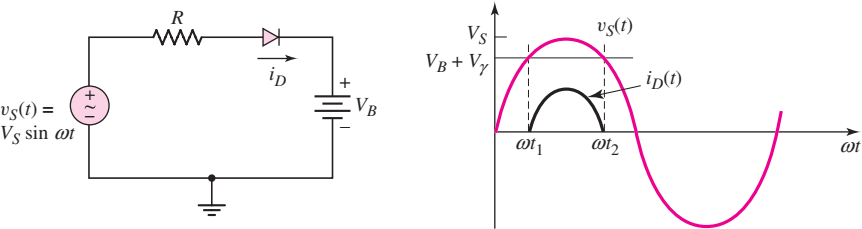
\includegraphics[width=\textwidth, height=9\baselineskip, keepaspectratio=true]{ds1}
\end{center}
\begin{align}
    i_D(\text{peak}) 
      &= \frac{V_S - V_B - V_\gamma}{R} 
       = \frac{12V - 5V - 0.73V}{200\Omega} = 31.35mA
\\  i_D 
      &= i_D(\text{peak}) \sin \omega t 
       = 31.35mA \sin \omega t
\\  v_R(\text{max}) 
      &= V_S + V_B
       = 12V + 5V
       = 17V
\\  \omega t_1 
	  &= v_S^{-1}(V_B + V_\gamma) 
	   = \arcsin(\frac{V_B + V_\gamma}{v_S}) 
	   = \arcsin(\frac{5V + 0.73V}{12}) 
	   = 28.52^\circ 
\\	\omega t_2
	  &= v_S^{-1}(V_B + V_\gamma) 
	   = \text{supplement}(\omega t_1)
	   = 180^\circ - \omega t_1
	   = 180^\circ - 28.52^\circ
	   = 151.84^\circ
\\  \% t
	  &= \frac{\omega t_2 - \omega t_1}{360^\circ} 
	   = \frac{151.48^\circ - 28.52^\circ}{360^\circ}
	   = 0.341\overline{5}
	   = 34.16\%
\end{align}

The peak diode current is $i_D(\text{peak}) = 31.35mA$. 
 The maximum reverse-bias diode voltage is $v_R = 17V$, 
 and the fraction of each cycle that the diode is conducting is $\%t = 34.16\%$

\subsection{Validation}

\begin{center}
LTSpice Implementation (accurate with $< 1\%$ deviation from design result)
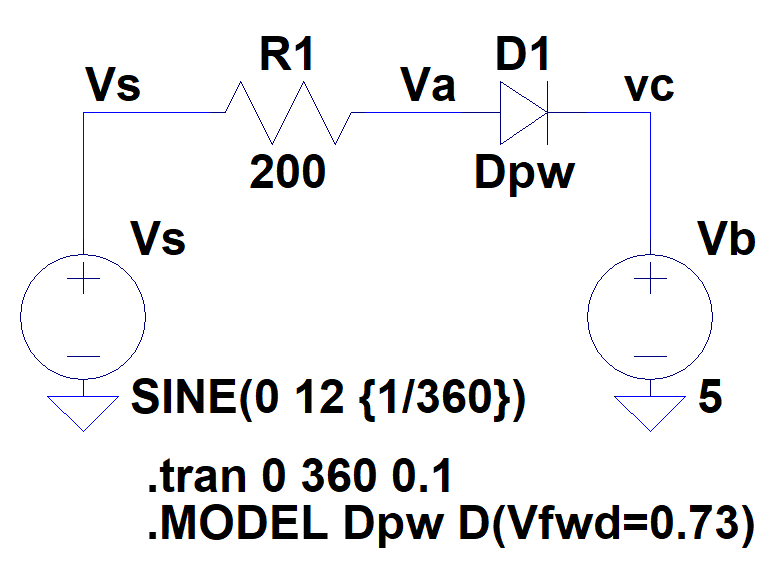
\includegraphics[width=.39\textwidth, height=\textheight, keepaspectratio=true]{ds1b}
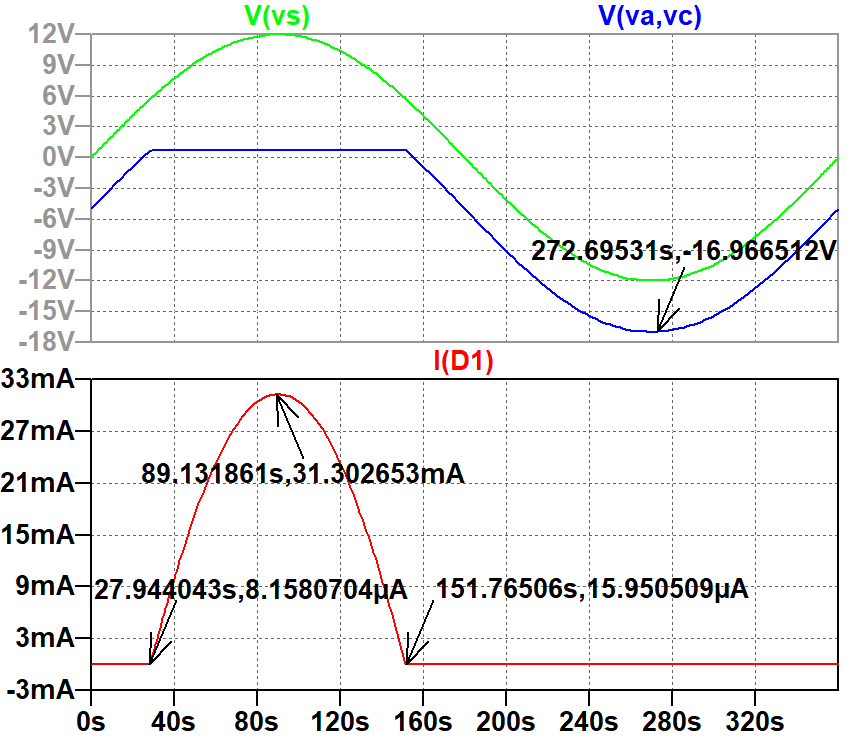
\includegraphics[width=.6\textwidth, height=\textheight, keepaspectratio=true]{ds1c}
\columnratio{0.5}
\begin{paracol}{2}
$Err_{V_R} = \frac{|17-16.966|}{17} = 0.002 = 0.2\%$
\switchcolumn
$Err_{i_D(\text{peak})} = \frac{|31.35-31.30|}{31.35} = 0.0015 = 0.15\%$
\switchcolumn
$Err_{\%t} = \frac{|0.3416-\frac{151.7-27.9}{360}|}{34.16} = 0.000007 = 0.00\%$
\switchcolumn
$Err_{Avg} = \frac{0.20 + 0.15 + 0.00}{3} = 0.12\%$
\end{paracol}
\end{center}

\clearpage
\section{Problem 7.2-1.b.1: } The problem is derived from problem 2.3 on page 112 of the textbook by changing the values, making $R$ dependent, and fixing the peak diode current. 
\subsection{Design}

A half-wave rectifier such as shown below has a peak diode current of $I_D = 2mA$.
The input is $V_I=120 V_{rms}$, $f=60 \text{Hz}$ signal and 
the transformer is a $10:1$ step down transformer.
The diode has a cut-in voltage of $V_\gamma = 1.2 V$.
Assume $r_f = 0$.

Determine the value of the resistor $R$,
 the peak output voltage,
 the fraction (percent) of a cycle that $v_O > 0$,
 the average output voltage, and
 the average current in the load.

\begin{center}
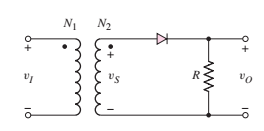
\includegraphics[width=\textwidth, height=7\baselineskip, keepaspectratio=true]{ds2}
\end{center}

\begin{align}
    \omega 
    	&= 120\pi
\\  v_I 
    	&= 120 V_{rms} 
         = 120\sqrt{2} V \sin(\omega t)
\\  v_S 
		&= \frac{1}{10}120\sqrt{2} V \sin(\omega t)
	     = 12\sqrt{2} V \sin(120\pi t)
\\  I_D
	    &= \frac{v_S - v_\gamma}{R}
\\ \implies R
		&= \frac{v_S - v_\gamma}{I_D}
		 = \frac{12\sqrt{2} - 1.2V}{2mA}
		 = 7885\Omega
\end{align}
\begin{align}
    \omega t_1 
	  &= v_S^{-1}(V_\gamma) 
	   = \arcsin(\frac{V_\gamma}{v_S}) 
	   = \arcsin(\frac{1.2V}{12\sqrt{2}V}) 
	   = 4.055^\circ 
\\	\omega t_2
      &= v_S^{-1}(V_\gamma)
	   = \text{supplement}(\omega t_1)
	   = 180^\circ - \omega t_1
       = 180^\circ - 4.055^\circ
       = 175.945^\circ
\\  \% t
	  &= \frac{\omega t_2 - \omega t_1}{360^\circ} 
	   = \frac{175.945^\circ - 4.055^\circ}{360^\circ}
	   = 0.47747\overline{2}
	   = 47.75\%
\\  V_O 
      &= V_S - V_\gamma
       = 12\sqrt{2}V - 1.2V
       = 15.77V
\\  v_O 
      &= V_O \sin(\omega t)
       = 15.77V \sin(\omega t)
\\  v_{O \text{avg}}
      &= \frac{V_O}{\omega} \int_{\omega t_1}^{\omega t_2} \sin(\omega t) d\omega t
       = \frac{15.77V}{2\pi} \int_{4.055^\circ}^{175.945^\circ} \sin(\omega t) d\omega t
       = 5.0075 V
\\  i_L
      &= i_D
       = 2 mA \sin(120\pi t)
\\  i_{L \text{avg}}
      &= \frac{I_L}{\omega} \int_{\omega t_1}^{\omega t_2} \sin(\omega t) d\omega t
       = \frac{2mA}{2\pi} \int_{4.055^\circ}^{175.945^\circ} \sin(\omega t) d\omega t
       = 635.1 \mu A
\end{align}

The the value of the resistor is $R = 7885\Omega$,
 the peak output voltage is $V_O = 15.77V$,
 the fraction (percent) of a cycle that $v_O > 0$ is $\%t = 47.75$,
 the average output voltage is $V_{O \text{avg}} = 5.0075 V$, and
 the average current in the load is $I_{L \text{avg}} = 635.1 \mu A$.

\clearpage
\subsection{Validation}

\begin{center}
LTSpice Implementation

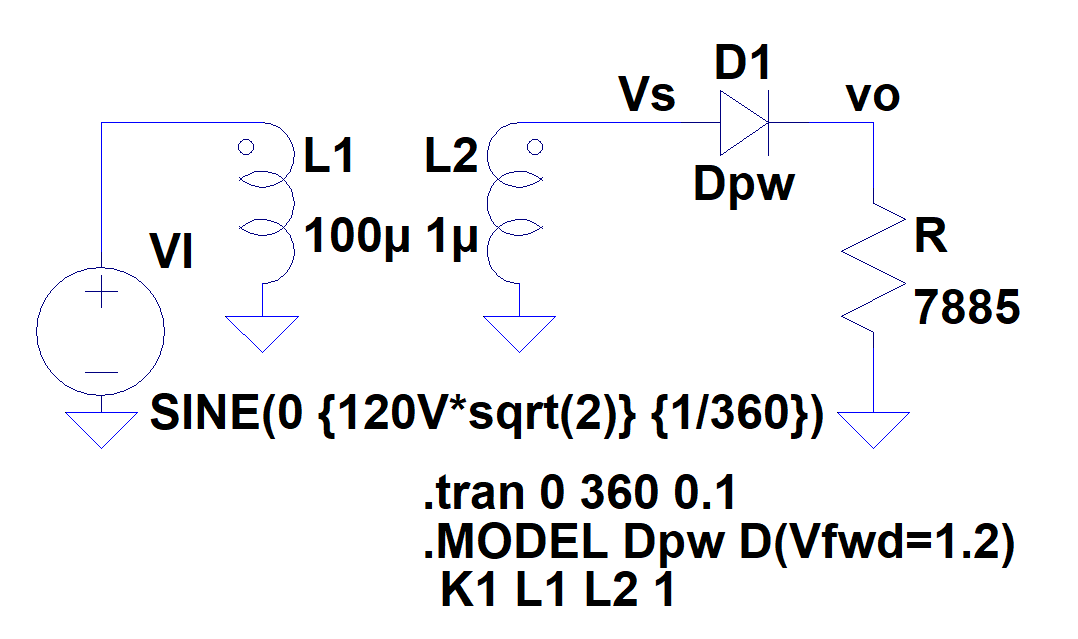
\includegraphics[width=.4\textwidth, height=\textheight, keepaspectratio=true]{ds2b}
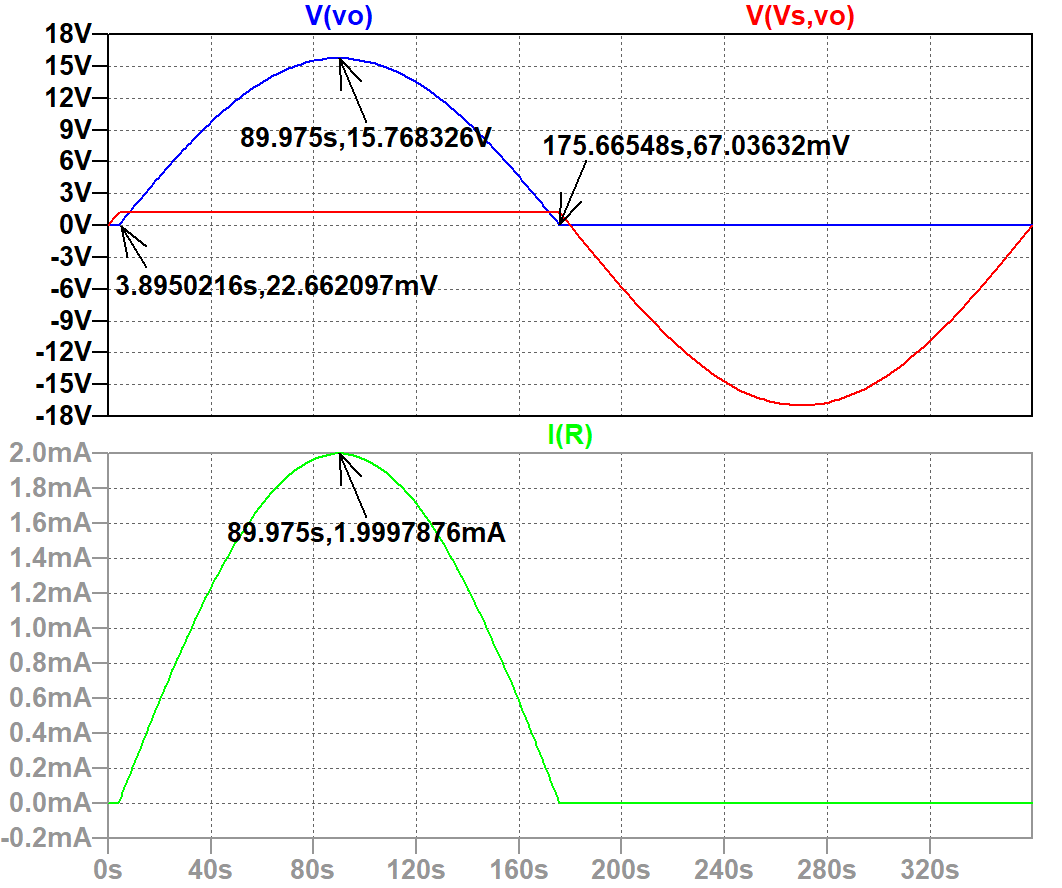
\includegraphics[width=.49\textwidth, height=\textheight, keepaspectratio=true]{ds2c}
\columnratio{0.6}
\begin{paracol}{2}
$Err_{V_O} = \frac{|15.77-15.768|}{15.77} = 0.01\%$
\switchcolumn
$Err_{V_{O \text{avg}}} = \frac{|5.0075-4.817|}{5.0075} = 3.80\%$
\switchcolumn
$Err_{I_{L \text{avg}}} = \frac{|635.1-610.91|}{635.1} = 3.80\%$
\switchcolumn
$Err_{\%t} = \frac{|0.4775-\frac{175.665 - 3.895}{360}|}{0.4775} = 0.08\%$
\switchcolumn
$Err_{Avg} = \frac{0.01 + 3.80 + 3.80 + 0.08}{4} = 1.92\%$
\end{paracol}
Error above $1\%$ is due to measurement error.
\end{center}

This assignment should demonstrate a basic understanding of manipulating basic half wave diode rectification circuits.

\textit{I have neither given nor received unauthorized assistance on this assignment.}


\end{raggedright}
\end{document}
